% Risk Lab: credit risk on a synthetic loan book - draft.
% Figures and tables are generated by report/build_report.py --doc credit (synthetic data only).
% Every \usertext{...} is an open prose slot for the author; a build with open slots is a draft.
\documentclass[11pt,a4paper]{article}
\usepackage[a4paper,margin=2.3cm]{geometry}
\usepackage{graphicx}
\usepackage[dvipsnames]{xcolor}
\usepackage{booktabs}
\usepackage{array}
\usepackage{amsmath,amssymb}
\usepackage{caption}
\usepackage{float}
\usepackage[hidelinks]{hyperref}
\captionsetup{font=small,labelfont=bf}
\graphicspath{{./}}

% Reproducible PDF: no creation date, empty trailer ID (pdfTeX primitives).
\ifdefined\pdfinfoomitdate \pdfinfoomitdate=1 \fi
\ifdefined\pdftrailerid \pdftrailerid{} \fi

% ---- open text slots ---------------------------------------------------------------
\newcounter{usertextslots}
\newcommand{\usertext}[1]{%
  \stepcounter{usertextslots}%
  \par\medskip\noindent
  \fcolorbox{BurntOrange}{Goldenrod!18}{\parbox{\dimexpr\linewidth-2\fboxsep-2\fboxrule\relax}{%
    \small\textbf{\textcolor{BurntOrange}{TEXT SLOT \theusertextslots:}} \textit{#1}}}%
  \par\medskip}
\makeatletter
\AtEndDocument{\immediate\write\@auxout{\string\gdef\string\totalusertextslots{\theusertextslots}}}
\makeatother
\providecommand{\totalusertextslots}{?}

\title{Credit risk on a synthetic loan book\\[0.3em]
  \large PD model validation, IFRS 9 expected credit loss and Basel IRB capital}
\author{}
\date{}

\begin{document}
\maketitle
\vspace{-2em}
\usertext{Author, function and date of the analysis.}
\begin{center}
\fcolorbox{BrickRed}{BrickRed!8}{\parbox{0.9\linewidth}{\centering\small
\textbf{DRAFT} -- this version has \totalusertextslots{} open text slots (orange boxes).
All figures and tables are generated from synthetic data by \texttt{report/build\_report.py --doc credit}.}}
\end{center}
\tableofcontents

% =====================================================================================
\section{Executive summary}
This document builds and checks the three standard pieces of a bank's credit-risk toolkit on a synthetic loan book
whose true default probabilities and default correlation are known: a probability-of-default (PD) model with its
validation tests, the IFRS 9 expected credit loss (ECL) with staging and macro scenarios, and the Basel IRB capital
requirement with its one-factor (Vasicek) foundation. Because the truth is known, the study can show where the
standard tests and formulas are reliable and where they mislead. The findings are in Table~\ref{tab:C6_findings};
their severities are proposals.
\usertext{The overall conclusion in two or three sentences, with the finding IDs.}

% =====================================================================================
\section{Data and scope}
Each period has a cross-section of borrowers with leverage, interest coverage, size, sector and an observable macro
variable. The true one-year PD is a logistic function of these features with known coefficients. Defaults follow a
one-factor Gaussian copula with asset correlation 0.12: a latent, unobservable systematic factor moves the default
rate of a whole period up or down, so defaults are correlated as in real portfolios. All modelling choices and
parameter sources are listed in the assumptions register (Table~\ref{tab:C5_assumptions}).

Not covered: retail and specialised-lending risk-weight functions, the SME firm-size adjustment, defaulted
exposures, credit risk mitigation, LGD and EAD estimation from data, and IFRS 9 modifications or purchased
credit-impaired assets.
\usertext{Which portfolio the synthetic book is meant to represent, and what a real-data version would need.}

% =====================================================================================
\section{PD model}
The model is a logistic regression estimated by maximum likelihood (Newton--Raphson); separation and
non-convergence stop the fit with an explicit error instead of a silently regularised result. Discrimination is
measured out of time by the AUC (the Mann--Whitney statistic) and the Gini / accuracy ratio; calibration by the
Hosmer--Lemeshow test, the Brier score and, per grade of a 9-grade master scale, the binomial and the Jeffreys tests.

\begin{figure}[H]
\centering
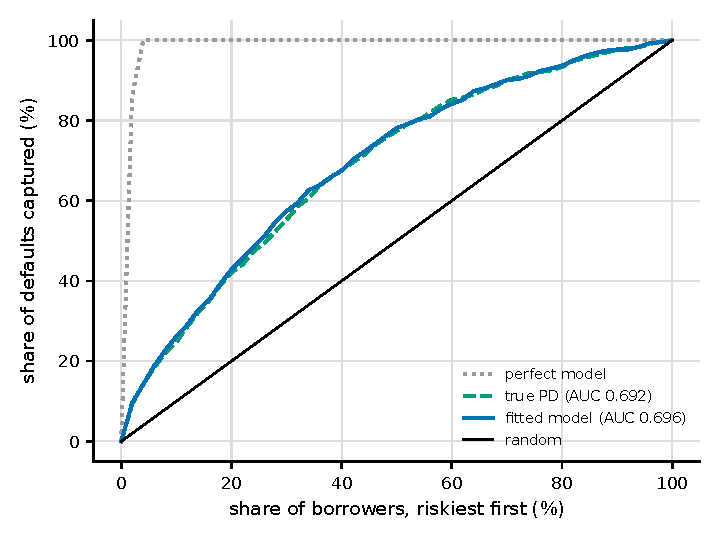
\includegraphics[width=0.6\linewidth]{figures/fig18_cap_roc.pdf}
\caption{Cumulative accuracy profile out of time (3 later periods) of the logistic PD model fitted on 50000 borrower-years, against the true PD and a perfect model (synthetic data). The model reaches the discrimination of the true PD (Gini 0.391); the true PD itself is far from perfect because defaults are random given the PD.}
\label{fig:fig18_cap_roc}
\end{figure}

\begin{table}[H]
\centering
\scriptsize
\caption{Logistic PD model. Top: one fit on 50000 borrower-years against the true coefficients (standard errors from the MLE information matrix; $z$ = (estimate $-$ true) / se). Bottom: out-of-time quality against the training size (M = 200 replications, $\pm$ Monte-Carlo se); failed = fits stopped with an explicit separation error. Failed fits are EXCLUDED: all averages are conditional on a successful fit. Macro: standard deviation of the macro coefficient over the successful fits / mean MLE standard error.}
\label{tab:C1_pd_model}
\setlength{\tabcolsep}{4pt}
\begin{tabular}{lrrrrr}
\toprule
Coefficient & True & Estimate & SE & $z$ &  \\
\midrule
const & -4.00 & -4.341 & 0.177 & -1.92 &  \\
leverage & +2.50 & +2.689 & 0.179 & +1.06 &  \\
log\_icr & -0.90 & -0.849 & 0.063 & +0.81 &  \\
log\_size & -0.25 & -0.264 & 0.037 & -0.37 &  \\
sector\_1 & +0.40 & +0.566 & 0.090 & +1.85 &  \\
sector\_2 & -0.30 & -0.077 & 0.103 & +2.18 &  \\
macro & -0.45 & -0.356 & 0.029 & +3.21 &  \\
\midrule
\textit{N train} & \textit{failed} & \textit{AUC} & \textit{gap to true} & \textit{coef.\ RMSE} & \textit{macro: sd / se} \\
500 & 74 & 0.675 $\pm$ 0.007 & +0.072 $\pm$ 0.007 & 1.594 $\pm$ 0.192 & 2.678 / 1.074 \\
2000 & 4 & 0.710 $\pm$ 0.005 & +0.036 $\pm$ 0.004 & 0.788 $\pm$ 0.039 & 1.478 / 0.499 \\
10000 & 0 & 0.714 $\pm$ 0.005 & +0.029 $\pm$ 0.005 & 0.547 $\pm$ 0.037 & 1.252 / 0.229 \\
50000 & 0 & 0.730 $\pm$ 0.004 & +0.018 $\pm$ 0.004 & 0.421 $\pm$ 0.023 & 1.026 / 0.087 \\
\bottomrule
\end{tabular}
\end{table}

\begin{figure}[H]
\centering
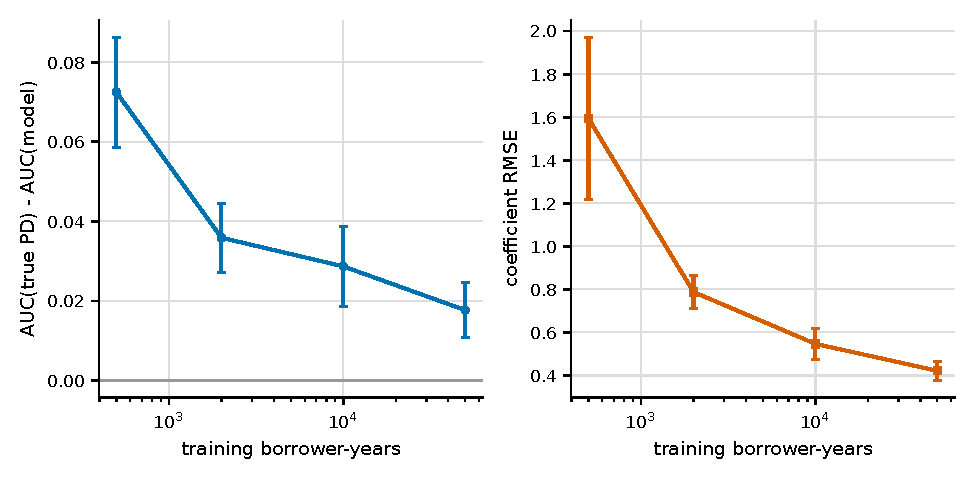
\includegraphics[width=\linewidth]{figures/fig19_pd_sample_size.pdf}
\caption{PD model quality against the training sample size (M = 200 replications per point, out-of-time test on 30\,000 borrower-years; error bars $\pm 1.96$ se). Left: the AUC lost against the true PD; right: the error of the estimated coefficients. Fits that failed with an explicit separation error are excluded and counted (74 at 500, 4 at 2000).}
\label{fig:fig19_pd_sample_size}
\end{figure}

\usertext{How much data a real model of this kind would need, and how the failed fits should be handled.}

\section{Calibration under correlated defaults and a macro shift}
\begin{table}[H]
\centering
\scriptsize
\caption{Top: rejection rates (\%, level 5\,\%) of calibration tests applied to the TRUE PD of one period of 20000 borrowers (M = 200), with independent defaults (asset correlation 0) and with asset correlation 0.12. Hosmer--Lemeshow: 10 groups, chi-square with 10 degrees of freedom (the true PD is not fitted on the sample; $g-2$ applies only to the development sample of a fitted model). The per-grade tests reject if any grade with at least 50 borrowers does (a multiple test over about 8 grades). Bottom: a downturn period (macro variable at -2 sd), \% $\pm$ Monte-Carlo se.}
\label{tab:C2_calibration}
\begin{tabular}{lrr}
\toprule
Test & Correlation 0 & Correlation 0.12 \\
\midrule
Hosmer--Lemeshow & 5.5 $\pm$ 1.6 & 82.5 $\pm$ 2.7 \\
binomial, any grade & 27.5 $\pm$ 3.2 & 36.0 $\pm$ 3.4 \\
Jeffreys, any grade & 34.5 $\pm$ 3.4 & 38.5 $\pm$ 3.4 \\
\midrule
\textit{Downturn} & \textit{predicted PD: mean (median)} & \textit{realised DR} \\
true PD & 3.55 $\pm$ 0.00 (3.55) & 3.65 $\pm$ 0.20 \\
model with macro & 5.46 $\pm$ 0.67 (3.22) & 3.65 $\pm$ 0.20 \\
model without macro & 1.65 $\pm$ 0.05 (1.54) & 3.65 $\pm$ 0.20 \\
\bottomrule
\end{tabular}
\end{table}

\begin{figure}[H]
\centering
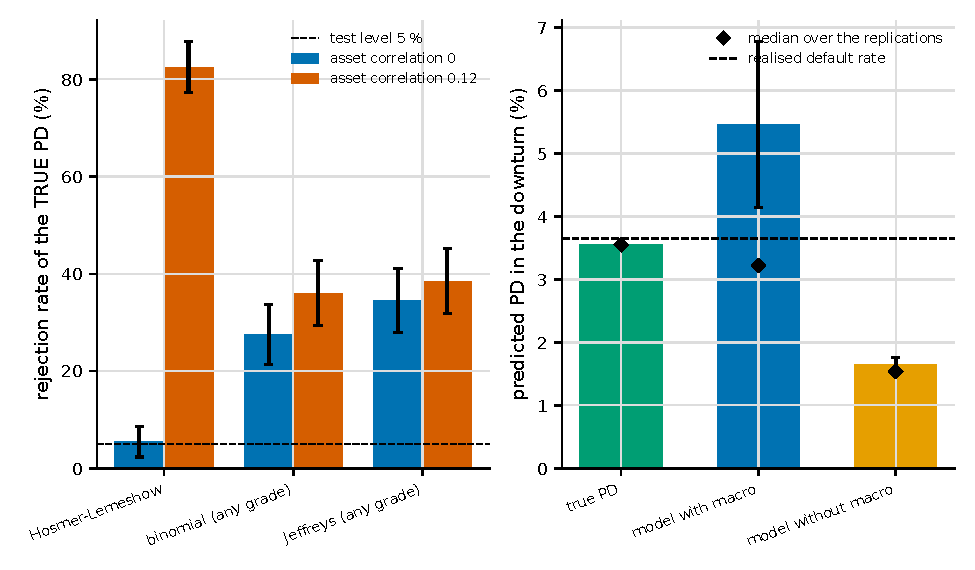
\includegraphics[width=\linewidth]{figures/fig20_calibration_drift.pdf}
\caption{Left: rejection rates of calibration tests applied to the TRUE PD of one period (20000 borrowers, M = 200), with independent defaults and with asset correlation 0.12; the per-grade tests reject if any grade does (multiple testing). Right: a downturn period (macro variable at -2 sd): mean (bars) and median (diamonds) predicted PD of the true model and of two fitted models (8 training periods) against the realised default rate; the mean of the model with the macro variable lies above its median (a noisy coefficient enters through the exponential). Hosmer--Lemeshow uses $g = 10$ degrees of freedom (the true PD is not fitted on the sample). Error bars $\pm 1.96$ se.}
\label{fig:fig20_calibration_drift}
\end{figure}

The Hosmer--Lemeshow statistic is compared with a chi-square distribution with $g = 10$ degrees of freedom: the
true PD (and a model applied out of time) is not fitted on the sample, and $g - 2$ applies only to the development
sample of a fitted model. With independent defaults the test then rejects the true PD at about its 5\,\% level;
with the realistic asset correlation it rejects the true PD in most periods, because a single year's default rate
carries the systematic factor. The per-grade binomial and Jeffreys tests are a multiple test: they reject in about a
third of the periods even without correlation, because about eight grades are tested at once, and correlation adds
comparatively little. In a downturn, a model without the macro variable underestimates the default rate; a model
whose macro sensitivity is estimated from few periods overshoots on average, but its median prediction is close to
the truth -- the noisy coefficient enters through the exponential (a Jensen effect).
\usertext{Which calibration tests and levels a validation function should use for such a model.}

% =====================================================================================
\section{IFRS 9 expected credit loss}
Stage 1 loans carry a 12-month ECL. Stage 2 loans carry a lifetime ECL; the trigger is a significant increase in
credit risk, here the current 12-month PD reaching a multiple of its value at origination (both compared on the
same basis, as base-scenario PDs without the scenario overlay, so the scenarios change the amount but not the
stage), or 30 days past due. Stage 3 loans (90 days past due) carry $\text{LGD} \times \text{EAD}$. The lifetime PD has a constant hazard per year, scaled by the
scenario's multipliers (upside, base, downside with weights), the exposure amortises, and the losses are discounted
at the effective interest rate. Deliberate simplifications: the exposure of a year is the balance at its start while
the default is assumed at its end; the stage-3 ECL is undiscounted; the hazard is constant over the lifetime.

\begin{table}[H]
\centering
\scriptsize
\caption{IFRS 9 ECL coverage (\% of EAD) of the synthetic book of 2000 loans by the weight of the downside scenario (rows; upside fixed at 20\,\%, base = the rest) and the relative SICR threshold (columns); in brackets the share of loans in stage 2 (\%). The SICR test compares the current and the origination 12-month PD on the same basis (both without the scenario overlay), so the stage-2 share depends on the threshold only. Deterministic.}
\label{tab:C3_ecl}
\setlength{\tabcolsep}{4pt}
\begin{tabular}{lrrrrrr}
\toprule
Downside weight & SICR $\times$1.5 & SICR $\times$2 & SICR $\times$2.5 & SICR $\times$3 & SICR $\times$4 & SICR $\times$5 \\
\midrule
0\,\% & 1.52 (30) & 1.29 (16) & 1.17 (9) & 1.09 (6) & 1.02 (3) & 0.97 (2) \\
10\,\% & 1.58 (30) & 1.34 (16) & 1.22 (9) & 1.13 (6) & 1.07 (3) & 1.02 (2) \\
20\,\% & 1.63 (30) & 1.40 (16) & 1.27 (9) & 1.18 (6) & 1.12 (3) & 1.07 (2) \\
30\,\% & 1.68 (30) & 1.45 (16) & 1.32 (9) & 1.23 (6) & 1.17 (3) & 1.12 (2) \\
40\,\% & 1.74 (30) & 1.50 (16) & 1.36 (9) & 1.28 (6) & 1.21 (3) & 1.16 (2) \\
50\,\% & 1.79 (30) & 1.55 (16) & 1.41 (9) & 1.33 (6) & 1.26 (3) & 1.21 (2) \\
60\,\% & 1.84 (30) & 1.60 (16) & 1.46 (9) & 1.37 (6) & 1.31 (3) & 1.26 (2) \\
\bottomrule
\end{tabular}
\end{table}

\begin{figure}[H]
\centering
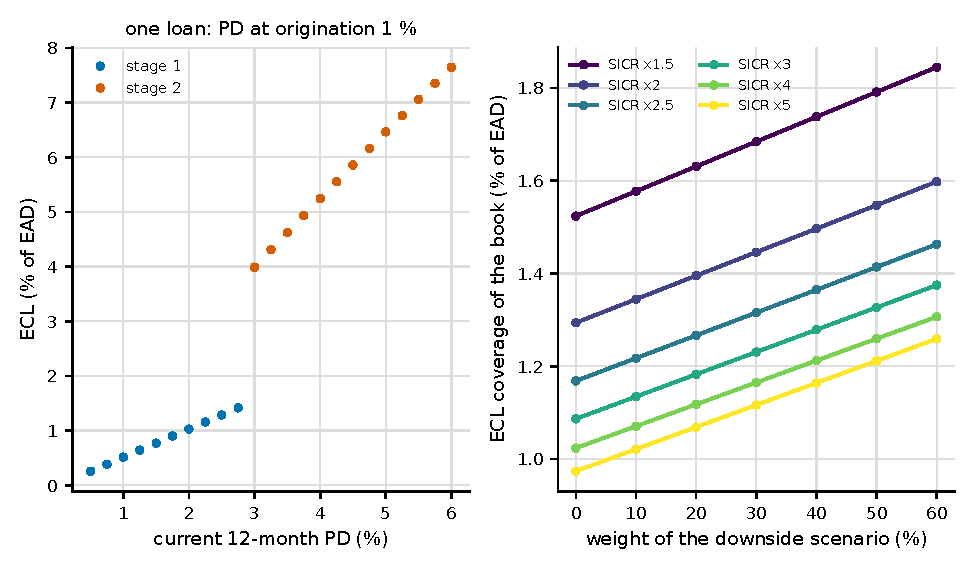
\includegraphics[width=\linewidth]{figures/fig21_ecl_cliff.pdf}
\caption{IFRS 9 ECL. Left: the stage-2 cliff of one 5-year amortising loan (PD at origination 1\,\%, LGD 45\,\%, EIR 5\,\%): when its current 12-month PD reaches 3 times the origination PD (both base-scenario PDs, the same basis) the provision jumps from 12-month to lifetime ECL. Right: the ECL coverage of a synthetic book of 2000 loans against the downside-scenario weight, for several relative SICR thresholds; the weight changes the measurement, not the stage.}
\label{fig:fig21_ecl_cliff}
\end{figure}

\usertext{Which SICR threshold and scenario weights the author would defend, and how to back-test them.}

% =====================================================================================
\section{Basel IRB capital}
For corporate exposures the capital requirement per unit of exposure is
\[
K = \left[\text{LGD}\;N\!\left(\frac{G(\text{PD}) + \sqrt{R}\,G(0.999)}{\sqrt{1-R}}\right) - \text{PD}\cdot\text{LGD}\right]
\frac{1 + (M - 2.5)\,b}{1 - 1.5\,b},
\]
with the correlation $R = 0.12\,w + 0.24\,(1-w)$, $w = (1 - e^{-50\,\text{PD}})/(1 - e^{-50})$, the maturity adjustment
$b = (0.11852 - 0.05478 \ln \text{PD})^2$ and $\text{RWA} = 12.5\,K\,\text{EAD}$ (BCBS 2006, para 272; CRE31; CRR
Art.~153; the illustrative risk weights of Basel II Annex 5 / CRE99 are reproduced exactly). With $M = 1$ the maturity term is 1 and $K/\text{LGD} + \text{PD}$ is the 99.9\,\% quantile of the default rate of
an infinitely granular portfolio in the one-factor model. The study simulates that model directly.

\begin{table}[H]
\centering
\scriptsize
\caption{IRB capital (sum of K $\times$ EAD\, M = 1 year, no PD floor) against the one-factor loss distribution (2,000,000 draws; 95\,\% order-statistic interval of the quantile). Total EAD 10\,000, LGD 45\,\%; granular and concentrated portfolios share the PD mix 0.1--5\,\%; the homogeneous ones have PD 1\,\%.}
\label{tab:C4_irb}
\setlength{\tabcolsep}{4pt}
\begin{tabular}{lrrrrrr}
\toprule
Portfolio & Names & Sum K & EL & q$_{99.9}$ (95\,\% CI) & q$_{99.9}-$EL & Ratio \\
\midrule
granular & 10000 & 630.6 & 81.5 & 707.9 (702.5--713.7) & 626.4 & 0.993 \\
concentrated & 30 & 630.6 & 81.5 & 1147.5 (1147.5--1147.5) & 1066.0 & 1.691 \\
homogeneous 10 & 10 & 586.2 & 45.0 & 1350.0 (1350.0--1350.0) & 1305.0 & 2.226 \\
homogeneous 30 & 30 & 586.2 & 45.0 & 900.0 (900.0--900.0) & 855.0 & 1.458 \\
homogeneous 100 & 100 & 586.2 & 45.0 & 720.0 (720.0--720.0) & 675.0 & 1.151 \\
homogeneous 300 & 300 & 586.2 & 45.0 & 660.0 (645.0--660.0) & 615.0 & 1.049 \\
homogeneous 1000 & 1000 & 586.2 & 45.0 & 639.0 (634.5--643.5) & 594.0 & 1.013 \\
homogeneous 10000 & 10000 & 586.2 & 45.0 & 629.6 (623.7--634.5) & 584.6 & 0.997 \\
\bottomrule
\end{tabular}
\end{table}

\begin{figure}[H]
\centering
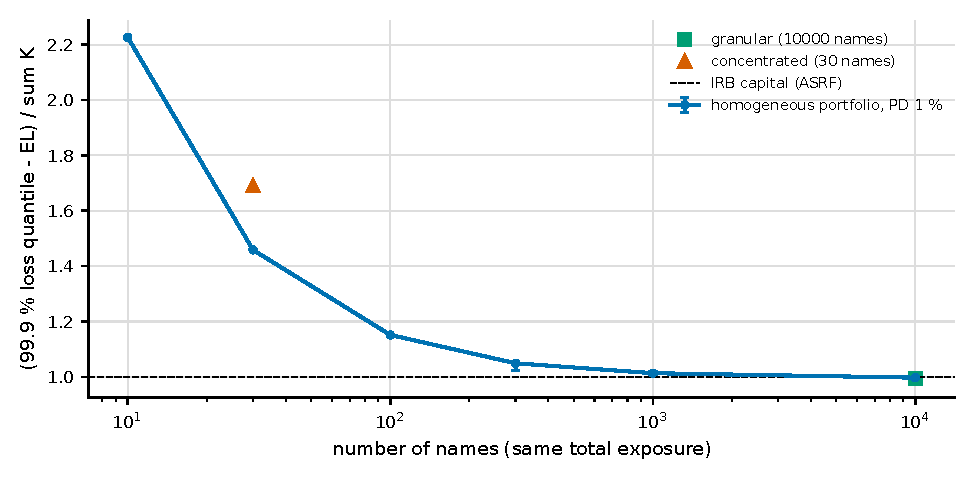
\includegraphics[width=\linewidth]{figures/fig22_irb_vs_mc.pdf}
\caption{IRB capital against the simulated one-factor loss distribution (2\,000,000 draws, M = 1 year so the maturity adjustment is 1, the IRB correlation of each PD). The ratio of the simulated 99.9\,\% quantile minus the expected loss to the sum of K is 1 for a large granular portfolio and grows as the exposure is concentrated in fewer names (name concentration is not in the IRB formula). Error bars: 95\,\% order-statistic intervals of the quantile.}
\label{fig:fig22_irb_vs_mc}
\end{figure}

\usertext{What a concentration add-on would look like for the bank's largest exposures.}

% =====================================================================================
\section{Limitations}
\begin{itemize}
\item Synthetic data: the conclusions illustrate the methods; the sizes depend on the chosen correlation, PD level and
  portfolio.
\item One correlation model (a single Gaussian factor); no contagion, no fat-tailed factors, no LGD--PD correlation.
\item Simple IFRS 9 models (constant lifetime hazards, scenario multipliers, constant LGD, exposure at the start of
  the year with default at its end, undiscounted stage-3 ECL); no forward-looking LGD.
\item Failed PD fits are excluded from the averages of Table~\ref{tab:C1_pd_model}, which are therefore conditional on
  a successful fit.
\item The order-statistic intervals of the 99.9\,\% loss quantile in Table~\ref{tab:C4_irb} collapse to a point for
  lumpy portfolios (few names): the loss takes few distinct values, so neighbouring order statistics coincide. This is
  expected, not a numerical error.
\item Regulatory parameters marked ``ASSUMPTION'' in Table~\ref{tab:C5_assumptions} must be verified before any use
  beyond this showcase.
\end{itemize}
\usertext{Further limitations the author sees.}

% =====================================================================================
\section{Findings}
\begin{table}[H]
\centering
\scriptsize
\caption{Findings register of the credit risk study. Severities are PROPOSED and must be confirmed by the validator.}
\label{tab:C6_findings}
\setlength{\tabcolsep}{3pt}
\begin{tabular}{>{\raggedright\arraybackslash}p{0.75cm}>{\raggedright\arraybackslash}p{6.6cm}>{\raggedright\arraybackslash}p{1.85cm}>{\raggedright\arraybackslash}p{2.4cm}>{\raggedright\arraybackslash}p{3.5cm}}
\toprule
ID & Finding & Severity & Evidence & Proposed remediation \\
\midrule
C-F1 & Calibration tests that assume independent defaults reject correct PDs in a single period: the Hosmer--Lemeshow test (chi-square with $g = 10$ degrees of freedom, as the true PD is not fitted on the sample) rejects the TRUE PD in 82.5 $\pm$ 2.7\,\% of the periods with asset correlation 0.12, against 5.5 $\pm$ 1.6\,\% (its nominal 5\,\%) with independent defaults; a one-year default rate carries the systematic factor. The per-grade binomial and Jeffreys tests are a multiple test over about 8 grades: they reject already with independent defaults (27.5 $\pm$ 3.2 / 34.5 $\pm$ 3.4\,\%), and correlation adds little (36.0 $\pm$ 3.4 / 38.5 $\pm$ 3.4\,\%). & PROPOSED: High & Tab.~\ref{tab:C2_calibration}; Fig.~\ref{fig:fig20_calibration_drift} & Interpret one-period calibration tests with correlation-adjusted critical values or over a cycle; control the family-wise level of per-grade tests (e.g. Bonferroni / Holm). \\
C-F2 & The MLE standard errors ignore the default correlation within a period: over the 200 replications with 50000 borrower-years (5 periods) the macro coefficient (true -0.45) has a spread of 1.026 (sd), 12 times its mean MLE standard error (0.087): the macro effect is identified from only 5 period-level observations, each shifted by the unobserved systematic factor. & PROPOSED: Medium & Tab.~\ref{tab:C1_pd_model} & Cluster standard errors by period, or estimate macro sensitivities on long histories. \\
C-F3 & In a downturn (macro at -2 sd) a model without the macro variable predicts 1.65 $\pm$ 0.05\,\% against a realised 3.65 $\pm$ 0.20\,\%. The model with the macro variable, estimated from 8 periods, overshoots on average (5.46 $\pm$ 0.67\,\%; true PD 3.55\,\%), but its median over the replications is 3.22\,\%: the overshoot of the mean is a Jensen effect - the noisy macro coefficient enters through the exponential, so the mean prediction is biased upwards; the median fit is close to the true PD. & PROPOSED: High & Tab.~\ref{tab:C2_calibration}; Fig.~\ref{fig:fig20_calibration_drift} & Monitor the calibration through the cycle; constrain macro sensitivities (expert bounds, longer data). \\
C-F4 & Small samples cost discrimination and stability: with 500 borrower-years 74 of 200 fits fail with separation, and the successful fits lose 0.072 AUC against the true PD; with 50000 the gap is 0.018. Failed fits are excluded, so the small-sample averages are conditional on success and flatter the model. & PROPOSED: Medium & Tab.~\ref{tab:C1_pd_model}; Fig.~\ref{fig:fig19_pd_sample_size} & Pool data or simplify the model for low-default portfolios; never hide failed fits. \\
C-F5 & The ECL depends strongly on two judgements: the coverage ranges from 0.97\,\% (no downside weight, SICR $\times$5) to 1.84\,\% (downside weight 60\,\%, SICR $\times$1.5). The SICR threshold moves the stage-2 share from 2 to 30\,\% and dominates; the downside weight changes the measurement only (staging compares PDs on the same basis, without the scenario overlay). The stage-2 transfer makes a single loan's provision jump by a multiple. & PROPOSED: Medium & Tab.~\ref{tab:C3_ecl}; Fig.~\ref{fig:fig21_ecl_cliff} & Disclose the sensitivity to the scenario weights and the SICR threshold; back-test the staging. \\
C-F6 & The IRB capital matches the one-factor 99.9\,\% loss of a granular portfolio (ratio 0.993) but understates a concentrated one: with 30 names the simulated unexpected loss is 1.69 times the sum of K. & PROPOSED: Medium & Tab.~\ref{tab:C4_irb}; Fig.~\ref{fig:fig22_irb_vs_mc} & Add a concentration charge (Pillar 2 / granularity adjustment) for portfolios with few names. \\
C-F7 & The IRB formula reproduces the illustrative risk weights of Basel II Annex 5 / CRE99 exactly, and the PD floor (CRE32.4), the M bounds (CRE32.46) and the CRR-only 1.06 scaling are confirmed; still used as recalled: the IFRS 9 paragraph numbers other than B5.5.13 and the ECB form of the Jeffreys test. & PROPOSED: Low & Tab.~\ref{tab:C5_assumptions} & Verify the remaining IFRS 9 references and the ECB instructions before any use beyond this showcase. \\
\bottomrule
\end{tabular}
\end{table}


\section{Assumptions register}
\begin{table}[H]
\centering
\scriptsize
\caption{Assumptions register of the credit study (``ASSUMPTION'' = not verified against a primary source in this work; ``stated'' = a modelling choice or a cited rule).}
\label{tab:C5_assumptions}
\setlength{\tabcolsep}{3pt}
\begin{tabular}{>{\raggedright\arraybackslash}p{3.0cm}>{\raggedright\arraybackslash}p{10.6cm}>{\raggedright\arraybackslash}p{2.1cm}}
\toprule
Item & Statement and source & Status \\
\midrule
IFRS 9 EAD & annual annuity balance at the start of each year (amortising) or full balance (bullet), with the default at the end of the year (simplification, slightly conservative) & stated \\
IFRS 9 LGD & constant per loan (synthetic parameter) & stated \\
IFRS 9 PD term structure & constant hazard = 12-month PD x scenario multiplier per year (simple model, synthetic) & stated \\
IFRS 9 backstop & 30 days past due: rebuttable presumption of SICR, IFRS 9 5.5.11 (as recalled) & stated \\
IFRS 9 default & 90 days past due: rebuttable presumption of default, IFRS 9 B5.5.37 (as recalled) & stated \\
IFRS 9 sicr proxy & 12-month PD change as a proxy for the lifetime PD change (IFRS 9 B5.5.13; confirmed in the v0.8 review) & stated \\
IFRS 9 stage 3 & ECL = LGD x EAD, undiscounted and without scenarios (simplification) & stated \\
IFRS 9 stages & IFRS 9 5.5.3 (lifetime if SICR) / 5.5.5 (12-month otherwise); paragraph numbers as recalled - ASSUMPTION & ASSUMPTION \\
IFRS 9 staging basis & current 12-month PD and the PD at origination compared on the same basis: both base-scenario PDs without the scenario overlay (modelling choice; scenarios affect the ECL, not the stage) & stated \\
IFRS 9 weighting & probability-weighted over scenarios, discounted at the EIR (IFRS 9 5.5.17 as recalled) & stated \\
IRB formula & BCBS (2006) Basel II para 272 / Basel Framework CRE31.4-31.5 / CRR Art. 153(1); reproduces the illustrative risk weights of Basel II Annex 5 and the CRE99 tables (14.44 / 29.65 / 92.32 \% at PD 0.03 / 0.10 / 1 \%, LGD 45 \%, M 2.5) exactly - confirmed in the v0.8 review & stated \\
IRB maturity & M floored at 1 and capped at 5 years (Basel Framework CRE32.46, confirmed in the v0.8 review; CRR Art. 162); parameters & stated \\
IRB not modelled & SME firm-size adjustment (CRE31.8), defaulted exposures, double default, credit risk mitigation & stated \\
IRB pd\_floor & 0.05 \% (Basel Framework CRE32.4; confirmed in the v0.8 review); parameter & stated \\
IRB scaling & 1.0 (Basel framework, CRE31); the 1.06 factor is CRR-only (CRR Art. 153(1)); parameter, default 1.0 & stated \\
Jeffreys test & ECB instructions for reporting the validation results of IRB models (2019), as recalled - ASSUMPTION; formula: Jeffreys-prior posterior & ASSUMPTION \\
data & synthetic: logit PD with known coefficients, one-factor Gaussian copula with asset correlation 0.12, observable AR(1) macro variable (modelling choices, not calibrations) & stated \\
master scale & 9 grades with PD bounds 0.1, 0.25, 0.5, 1, 2, 4, 8, 15 \% (synthetic) & stated \\
\bottomrule
\end{tabular}
\end{table}


\section*{References}
\begin{itemize}
\item Basel Committee on Banking Supervision (2006). \emph{International convergence of capital measurement and
  capital standards} (Basel II), paras 272 ff. and Annex 5 (illustrative IRB risk weights).
\item Basel Committee on Banking Supervision. \emph{The Basel Framework}, CRE31 (risk-weight functions), CRE32.4 (PD
  floor), CRE32.46 (effective maturity), CRE99 (illustrative risk weights).
\item Basel Committee on Banking Supervision (2005). \emph{An explanatory note on the Basel II IRB risk weight functions}.
\item Regulation (EU) No 575/2013 (CRR), Art.~153 (risk weights, 1.06 scaling) and Art.~162 (maturity).
\item IFRS 9 \emph{Financial Instruments}, section 5.5 (impairment).
\item Vasicek, O. (2002). The distribution of loan portfolio value. \emph{Risk} 15(12), 160--162.
\item Hosmer, D. W. and Lemeshow, S. (2000). \emph{Applied Logistic Regression}, 2nd ed. Wiley.
\item European Central Bank (2019). Instructions for reporting the validation results of internal models (IRB).
\end{itemize}

\appendix
\section{Reproduction}
From \texttt{UFOS.ai/RiskLab/}:
\begin{verbatim}
python studies/credit_risk.py --mode full --save-results
python report/build_report.py --doc credit
# -> out/report/credit.pdf
\end{verbatim}

\end{document}
